\subsection{Regularization}

Among all unbiased solutions $(X^TX)^{-1}X^TY$ is the solution that has the smallest variance $\Rightarrow$ minimizes gen. Error

However the variance can get big $\Rightarrow$ small $L_{train}(\omega)$ but large $L_{gen}(\omega)$ due to overfitting. Noise increases weights and regularization counters that effect. $\Rightarrow$ Regularization:

One can set the $\omega$ of higher order features manually to zero ($\leftrightarrow$ choose a less complex model) or

\textbf{Ridge Regression}

$\underset{\omega}{min}||Y-X\omega||^2 + \lambda||\omega||^2$

Always allows for closed solution and lets LS converge faster through better conditioned problem (EVs of Hessian $X^TX$ change)

Equivalent to performing Bayesianism approach with $p(\omega) = \mathcal{N}(\omega|0,\boldsymbol{\Lambda}^{-1})$ or linearly $p(\omega) = \mathcal{N}(\omega|0,1)$

Weights are decreased in general but not necessarily to exactly 0.

\textbf{Lasso Regression}

Not a convex loss $\Rightarrow$ no closed form solution

$\underset{\omega}{min}||Y-X\omega||^2 + \lambda|\omega|$

Equivalent to performing Bayesianism approach with Laplacian prior:  $p(\omega_i) = \frac{\lambda}{4\sigma^2}exp(-|\omega_i|\frac{\lambda}{w\sigma^2})$

The weights of higher complexity features go to absolute zero $\Rightarrow$ sparse weight vector result

\begin{center}
    \resizebox{0.6\linewidth}{!}{
    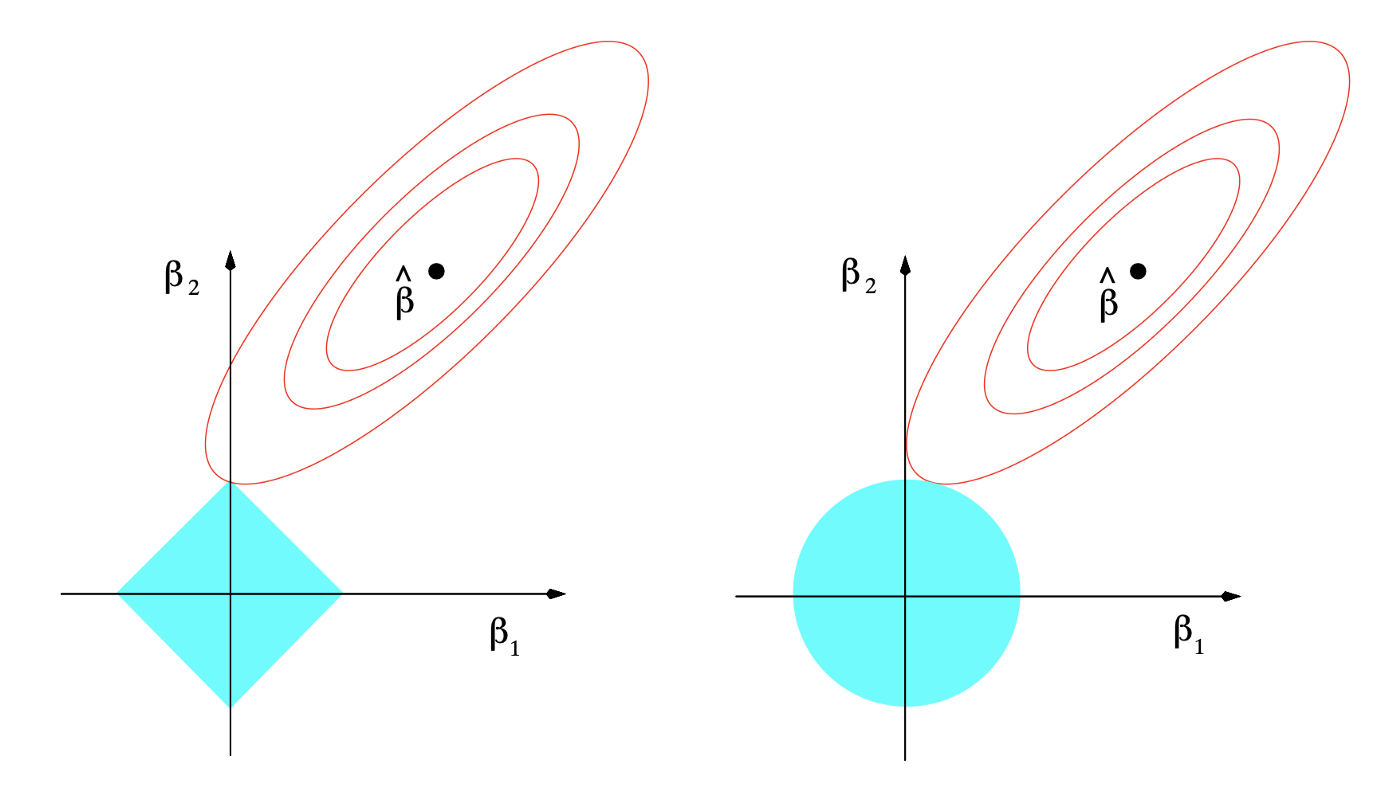
\includegraphics{images/lasso_vs_ridge.png}
    }
\end{center}
Left: Lasso, Right: Ridge

In general with increasing $\lambda$ the bias increases. $\lambda_{opt}$ can be found using CV.
